\documentclass[border=10pt]{standalone}
\usepackage{tikz}
\usepackage{xcolor}
\usetikzlibrary{positioning,arrows.meta,fit,backgrounds,calc}

\definecolor{C1}{RGB}{219,234,254}
\definecolor{C1b}{RGB}{37,99,235}
\definecolor{C2}{RGB}{254,243,199}
\definecolor{C2b}{RGB}{160,100,0}
\definecolor{C3}{RGB}{237,233,254}
\definecolor{C3b}{RGB}{109,40,217}
\definecolor{C4}{RGB}{209,250,229}
\definecolor{C4b}{RGB}{5,130,90}

\begin{document}
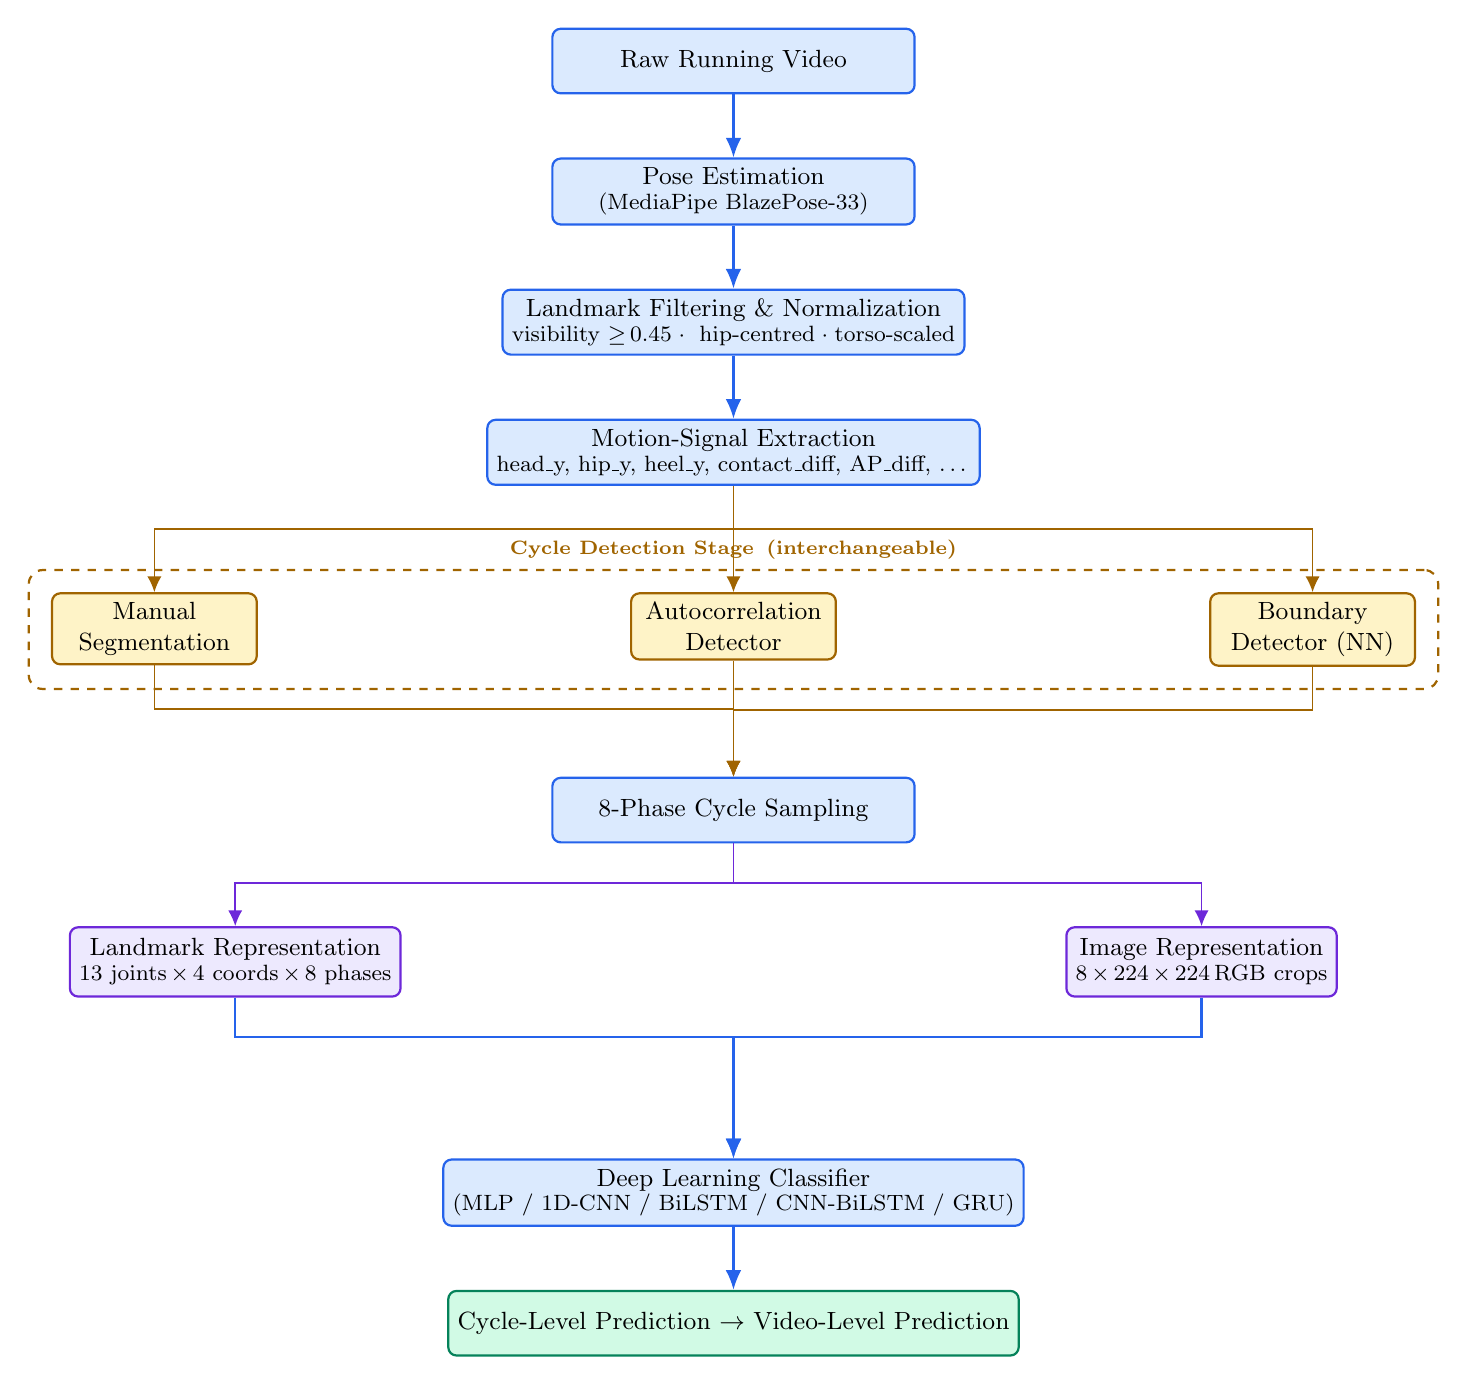
\begin{tikzpicture}[
  node distance = 0.8cm and 1.0cm,
  mainbox/.style = {
    rectangle, rounded corners=3pt,
    draw=C1b, fill=C1, thick,
    align=center, minimum width=4.6cm, minimum height=0.82cm,
    font=\small
  },
  altbox/.style = {
    rectangle, rounded corners=3pt,
    draw=C2b, fill=C2, thick,
    align=center, minimum width=2.6cm, minimum height=0.78cm,
    font=\small
  },
  reprbox/.style = {
    rectangle, rounded corners=3pt,
    draw=C3b, fill=C3, thick,
    align=center, minimum width=3.4cm, minimum height=0.88cm,
    font=\small
  },
  outbox/.style = {
    rectangle, rounded corners=3pt,
    draw=C4b, fill=C4, thick,
    align=center, minimum width=4.6cm, minimum height=0.82cm,
    font=\small
  },
  ma/.style  = {-{Latex[length=2.5mm,width=2mm]}, thick, C1b},
  ca/.style  = {-{Latex[length=2mm,width=1.8mm]}, semithick, C2b},
  ra/.style  = {-{Latex[length=2mm,width=1.8mm]}, semithick, C3b}
]

%% ---------- Main pipeline stages ----------
\node[mainbox] (vid)
    {Raw Running Video};

\node[mainbox, below=of vid] (pose)
    {Pose Estimation\\[-2pt]{\footnotesize (MediaPipe BlazePose-33)}};

\node[mainbox, below=of pose] (filt)
    {Landmark Filtering \& Normalization\\[-2pt]%
     {\footnotesize visibility ${\geq}$\,0.45\;$\cdot$\; hip-centred\;$\cdot$\;torso-scaled}};

\node[mainbox, below=of filt] (sig)
    {Motion-Signal Extraction\\[-2pt]%
     {\footnotesize head\_y, hip\_y, heel\_y, contact\_diff, AP\_diff, \ldots}};

%% ---------- Cycle Detection (three interchangeable variants) ----------
\node[altbox, below left=1.35cm and 2.9cm of sig]  (hand)
    {Manual\\Segmentation};
\node[altbox, below=1.35cm of sig]                  (auto)
    {Autocorrelation\\Detector};
\node[altbox, below right=1.35cm and 2.9cm of sig] (bdet)
    {Boundary\\Detector (NN)};

\begin{scope}[on background layer]
  \node[draw=C2b, dashed, rounded corners=5pt, thick,
        fit=(hand)(auto)(bdet), inner sep=8pt,
        label={[font=\scriptsize\bfseries\color{C2b}]above:%
               Cycle Detection Stage\enspace(interchangeable)}
       ] (cyc) {};
\end{scope}

%% ---------- After cycle detection ----------
\node[mainbox, below=1.1cm of cyc] (phase)
    {8-Phase Cycle Sampling};

\node[reprbox, below left=1.05cm and 1.9cm of phase]  (lm)
    {Landmark Representation\\[-2pt]{\footnotesize 13 joints\,$\times$\,4 coords\,$\times$\,8 phases}};

\node[reprbox, below right=1.05cm and 1.9cm of phase] (im)
    {Image Representation\\[-2pt]{\footnotesize 8\,$\times$\,224\,$\times$\,224\,RGB crops}};

\node[mainbox, below=4.0cm of phase] (cls)
    {Deep Learning Classifier\\[-2pt]{\footnotesize (MLP / 1D-CNN / BiLSTM / CNN-BiLSTM / GRU)}};

\node[outbox, below=of cls] (out)
    {Cycle-Level Prediction $\to$ Video-Level Prediction};

%% ---------- Arrows ----------
\draw[ma] (vid)  -- (pose);
\draw[ma] (pose) -- (filt);
\draw[ma] (filt) -- (sig);

% sig → cycle detection (fan out)
\draw[ca] (sig.south) -- ++(0,-0.55) -| (hand.north);
\draw[ca] (sig.south) -- ++(0,-0.55) -- (auto.north);
\draw[ca] (sig.south) -- ++(0,-0.55) -| (bdet.north);

% cycle detection → phase (fan in)
\draw[ca] (hand.south) -- ++(0,-0.55) -| (phase.north);
\draw[ca] (auto.south) -- ++(0,-0.55) -- (phase.north);
\draw[ca] (bdet.south) -- ++(0,-0.55) -| (phase.north);

% phase → representations (fork)
\draw[ra] (phase.south) -- ++(0,-0.5) -| (lm.north);
\draw[ra] (phase.south) -- ++(0,-0.5) -| (im.north);

% representations → classifier (merge)
\draw[ma] (lm.south) -- ++(0,-0.5) -| (cls.north);
\draw[ma] (im.south) -- ++(0,-0.5) -| (cls.north);

\draw[ma] (cls) -- (out);

\end{tikzpicture}
\end{document}
